\documentclass{article}
\usepackage{pgfplots}
\usepackage{filecontents}
\usepackage{tikz}
\usepackage{verbatim}
\pgfplotsset{compat=1.8}
\usepackage{pgfplotstable}

\begin{document}

%% \begin{tikzpicture}
%%   \draw (1,0) -- (0,0) -- (0,1);
%% \end{tikzpicture}

%% \begin{tikzpicture}
%% \draw[red, dashed, very thick, rotate=30] (1,0) -- (0,0) -- (0,1);
%% \end{tikzpicture}

%% \begin{tikzpicture}
%% \draw (1,0) -- (0,0) -- (0,1) -- cycle;
%% \end{tikzpicture}

%% \begin{tikzpicture}
%% \draw (0,0) -- (2,0) (0,1) -- (2,1);
%% \end{tikzpicture}

%% \begin{tikzpicture}
%% \draw (0,0) -- (3,1)
%% node[pos=0]{0} node[pos=0.5]{1/2} node[pos=0.9]{9/10};
%% \end{tikzpicture}

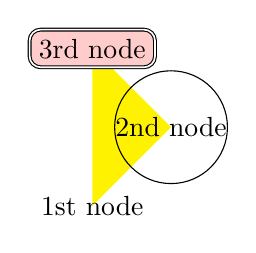
\begin{tikzpicture}
\fill[fill=yellow]
(0,0) node {1st node}
-- (1,1) node[circle,inner sep=0pt,draw] {2nd node}
-- (0,2) node[fill=red!20,draw,double,rounded corners] {3rd node};
\end{tikzpicture}

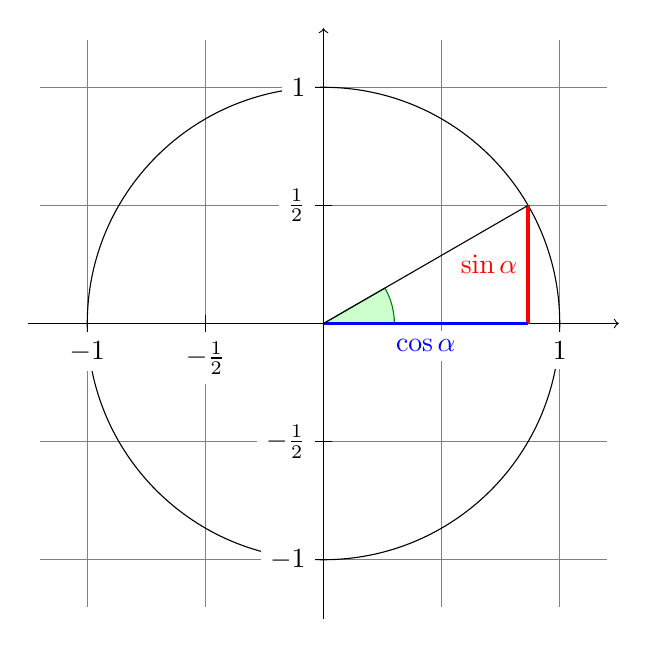
\begin{tikzpicture}[scale=3]
  \draw[step=.5cm, gray, very thin] (-1.2,-1.2) grid (1.2,1.2);
  \filldraw[fill=green!20,draw=green!50!black] (0,0) -- (3mm,0mm) arc (0:30:3mm) -- cycle;
  \draw[->] (-1.25,0) -- (1.25,0) coordinate (x axis); % -> makes axis
  \draw[->] (0,-1.25) -- (0,1.25) coordinate (y axis);
  \draw (0,0) circle (1cm);
  \draw[very thick,red] (30:1cm) -- node[left,fill=white] {$\sin \alpha$} (30:1cm |- x axis);
  \draw[very thick,blue] (30:1cm |- x axis) -- node[below=2pt,fill=white] {$\cos \alpha$} (0,0);
  \draw (0,0) -- (30:1cm);
  \foreach \x/\xtext in {-1, -0.5/-\frac{1}{2}, 1}
  \draw (\x cm,1pt) -- (\x cm,-1pt) node[anchor=north,fill=white] {$\xtext$};
  \foreach \y/\ytext in {-1, -0.5/-\frac{1}{2}, 0.5/\frac{1}{2}, 1}
  \draw (1pt,\y cm) -- (-1pt,\y cm) node[anchor=east,fill=white] {$\ytext$};
\end{tikzpicture}
\end{document}
